\section{Результаты}
\subsection{Выборочные коэффициенты корреляции}
\begin{table}[H]
	\centering
	\begin{tabular}{|c|c|c|c|}
\hline
$\rho = 0~(
\ref{ro})$ & $r ~(
\ref{r})$ & $r_Q ~(
\ref{rQ})$ & $r_S ~(
\ref{rS})$\\
\hline
$E(z)$ & -0.011 & -0.012 & -0.012\\
\hline
$E(z^2)$ & 0.055 & 0.055 & 0.054\\
\hline
$D(z)$ & 0.235 & 0.234 & 0.231\\
\hline
$\rho = 0.5~(
\ref{ro})$ & $r ~(
\ref{r})$ & $r_Q ~(
\ref{rQ})$ & $r_S ~(
\ref{rS})$\\
\hline
$E(z)$ & 0.477 & 0.451 & 0.323\\
\hline
$E(z^2)$ & 0.259 & 0.24 & 0.151\\
\hline
$D(z)$ & 0.179 & 0.19 & 0.215\\
\hline
$\rho = 0.9~(
\ref{ro})$ & $r ~(
\ref{r})$ & $r_Q ~(
\ref{rQ})$ & $r_S ~(
\ref{rS})$\\
\hline
$E(z)$ & 0.895 & 0.865 & 0.695\\
\hline
$E(z^2)$ & 0.804 & 0.754 & 0.512\\
\hline
$D(z)$ & 0.05 & 0.071 & 0.172\\
\hline
\end{tabular}
	\caption{Двумерное нормальное распределение, n = 20}
	\label{tab:n20}
\end{table}
\begin{table}[H]
	\centering
	\begin{tabular}{|c|c|c|c|}
\hline
$\rho = 0~(
\ref{ro})$ & $r ~(
\ref{r})$ & $r_Q ~(
\ref{rQ})$ & $r_S ~(
\ref{rS})$\\
\hline
$E(z)$ & -0.001 & 0.001 & 0.001\\
\hline
$E(z^2)$ & 0.018 & 0.017 & 0.017\\
\hline
$D(z)$ & 0.134 & 0.132 & 0.131\\
\hline
$\rho = 0.5~(
\ref{ro})$ & $r ~(
\ref{r})$ & $r_Q ~(
\ref{rQ})$ & $r_S ~(
\ref{rS})$\\
\hline
$E(z)$ & 0.495 & 0.474 & 0.333\\
\hline
$E(z^2)$ & 0.255 & 0.235 & 0.126\\
\hline
$D(z)$ & 0.098 & 0.103 & 0.122\\
\hline
$\rho = 0.9~(
\ref{ro})$ & $r ~(
\ref{r})$ & $r_Q ~(
\ref{rQ})$ & $r_S ~(
\ref{rS})$\\
\hline
$E(z)$ & 0.898 & 0.882 & 0.708\\
\hline
$E(z^2)$ & 0.807 & 0.78 & 0.51\\
\hline
$D(z)$ & 0.026 & 0.033 & 0.091\\
\hline
\end{tabular}
	\caption{Двумерное нормальное распределение, n = 60}
	\label{tab:n60}
\end{table}
\begin{table}[H]
	\centering
	\begin{tabular}{|c|c|c|c|}
\hline
$\rho = 0~(
\ref{ro})$ & $r ~(
\ref{r})$ & $r_Q ~(
\ref{rQ})$ & $r_S ~(
\ref{rS})$\\
\hline
$E(z)$ & 0.003 & 0.002 & 0.002\\
\hline
$E(z^2)$ & 0.01 & 0.01 & 0.01\\
\hline
$D(z)$ & 0.099 & 0.099 & 0.101\\
\hline
$\rho = 0.5~(
\ref{ro})$ & $r ~(
\ref{r})$ & $r_Q ~(
\ref{rQ})$ & $r_S ~(
\ref{rS})$\\
\hline
$E(z)$ & 0.495 & 0.476 & 0.335\\
\hline
$E(z^2)$ & 0.251 & 0.233 & 0.122\\
\hline
$D(z)$ & 0.079 & 0.084 & 0.1\\
\hline
$\rho = 0.9~(
\ref{ro})$ & $r ~(
\ref{r})$ & $r_Q ~(
\ref{rQ})$ & $r_S ~(
\ref{rS})$\\
\hline
$E(z)$ & 0.898 & 0.885 & 0.705\\
\hline
$E(z^2)$ & 0.807 & 0.784 & 0.503\\
\hline
$D(z)$ & 0.02 & 0.025 & 0.071\\
\hline
\end{tabular}
	\caption{Двумерное нормальное распределение, n = 100}
	\label{tab:n100}
\end{table}
\begin{table}[H]
	\centering
	\begin{tabular}{|c|c|c|c|}
\hline
$n = 20$ & $r ~(
\ref{r})$ & $r_Q ~(
\ref{rQ})$ & $r_S ~(
\ref{rS})$\\
\hline
$E(z)$ & 0.803 & 0.773 & 0.597\\
\hline
$E(z^2)$ & 0.653 & 0.609 & 0.391\\
\hline
$D(z)$ & 0.087 & 0.106 & 0.187\\
\hline
$n = 60$ & $r ~(
\ref{r})$ & $r_Q ~(
\ref{rQ})$ & $r_S ~(
\ref{rS})$\\
\hline
$E(z)$ & 0.809 & 0.788 & 0.594\\
\hline
$E(z^2)$ & 0.656 & 0.623 & 0.364\\
\hline
$D(z)$ & 0.045 & 0.055 & 0.106\\
\hline
$n = 100$ & $r ~(
\ref{r})$ & $r_Q ~(
\ref{rQ})$ & $r_S ~(
\ref{rS})$\\
\hline
$E(z)$ & 0.809 & 0.791 & 0.597\\
\hline
$E(z^2)$ & 0.656 & 0.628 & 0.363\\
\hline
$D(z)$ & 0.035 & 0.042 & 0.081\\
\hline
\end{tabular}
	\caption{Смесь нормальных распределений}
	\label{tab:mix}
\end{table}

\subsection{Эллипсы рассеивания}
\begin{flushleft}
	Для уравнения эллипса выбиралась константа $const = 9$.
\end{flushleft}
\begin{figure}[H]
	\center{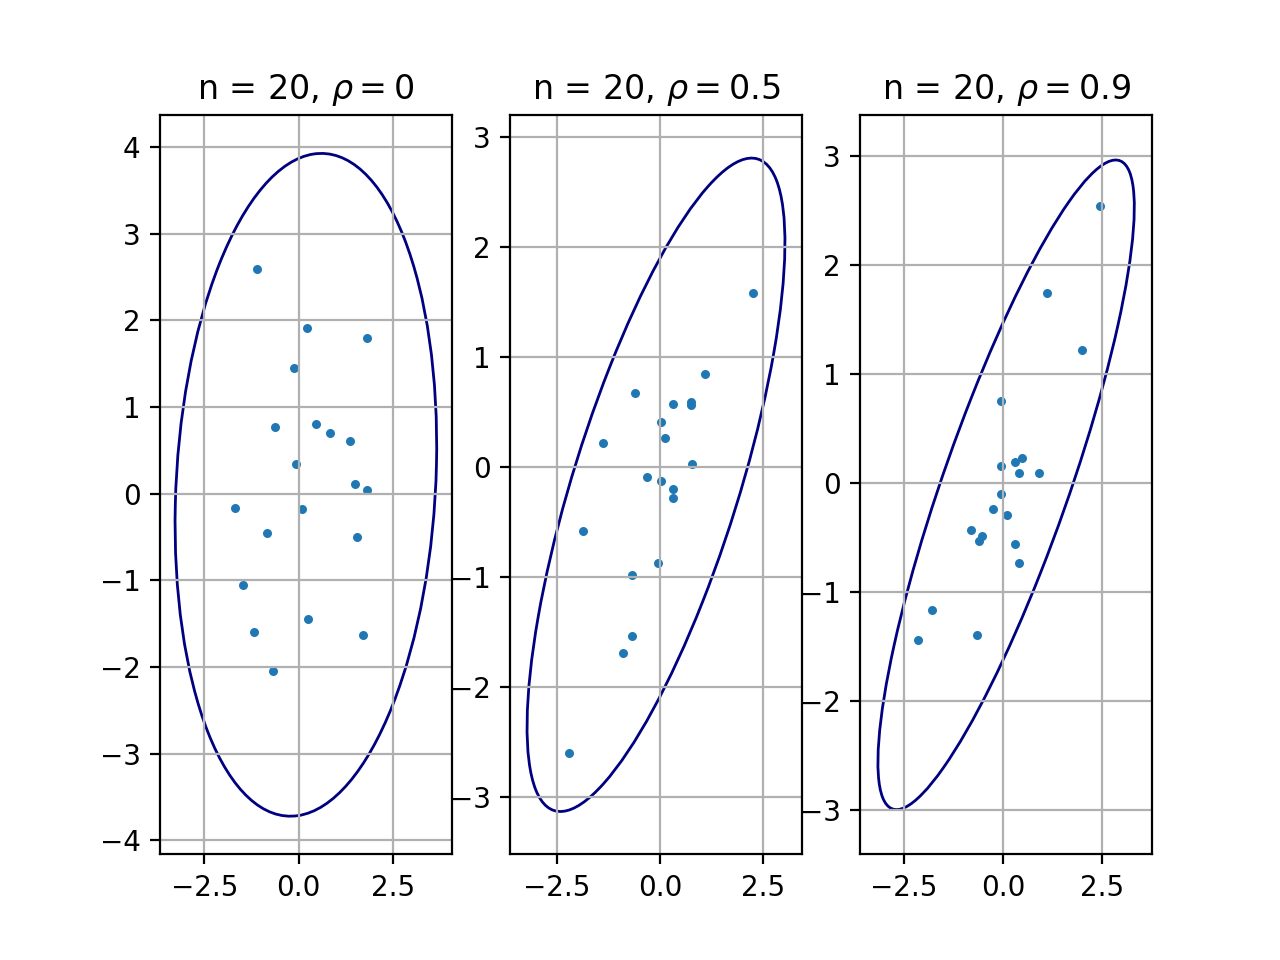
\includegraphics[width=1\linewidth]{task1\_data/20}}
	\caption{Двумерное нормальное распределение, $n$ = 20}
	\label{fig:n20}
\end{figure}
\begin{figure}[H]
	\center{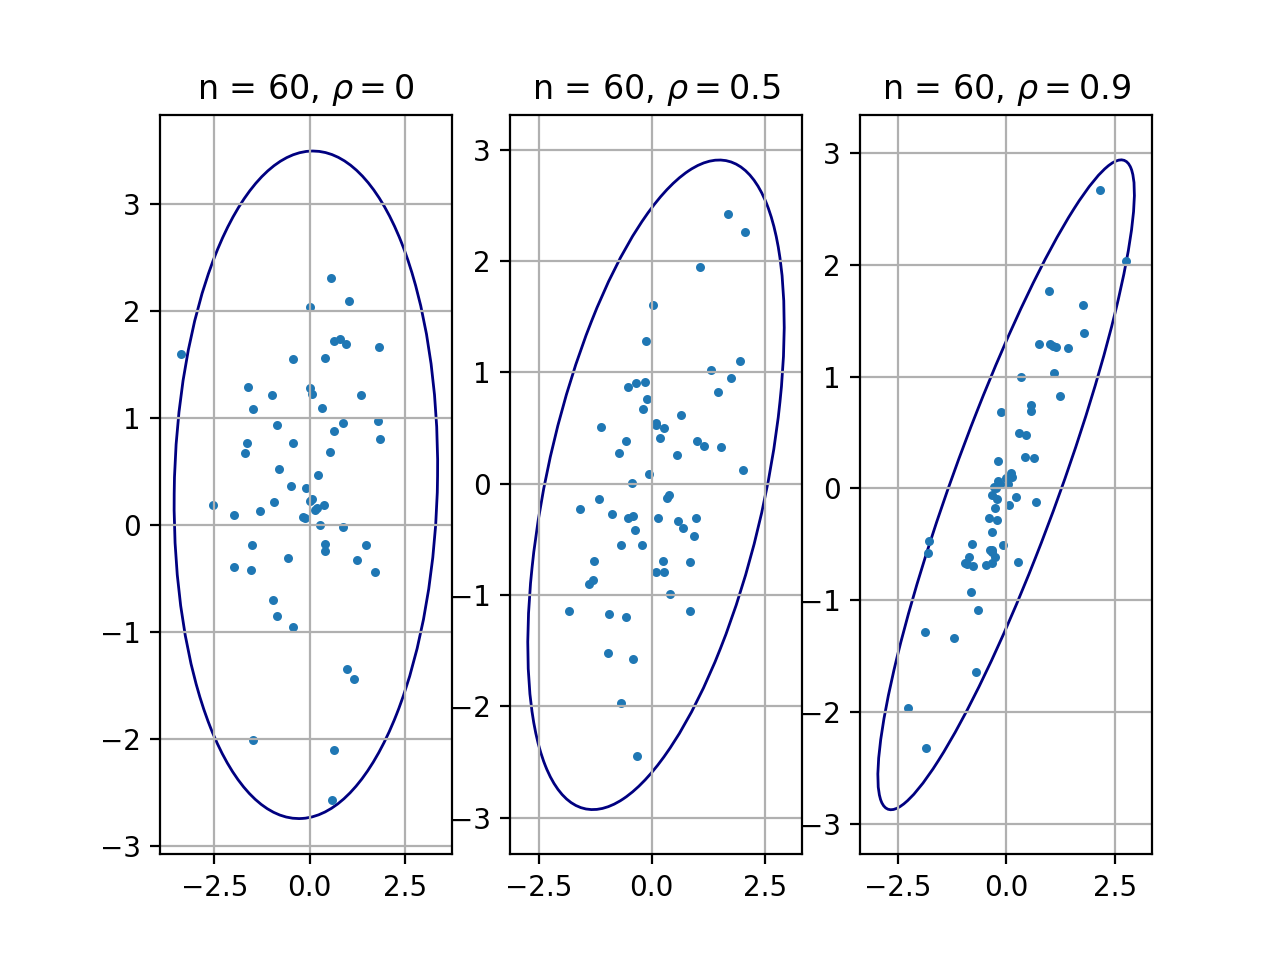
\includegraphics[width=1\linewidth]{task1\_data/60}}
	\caption{Двумерное нормальное распределение, $n$ = 60}
	\label{fig:n60}
\end{figure}
\begin{figure}[H]
	\center{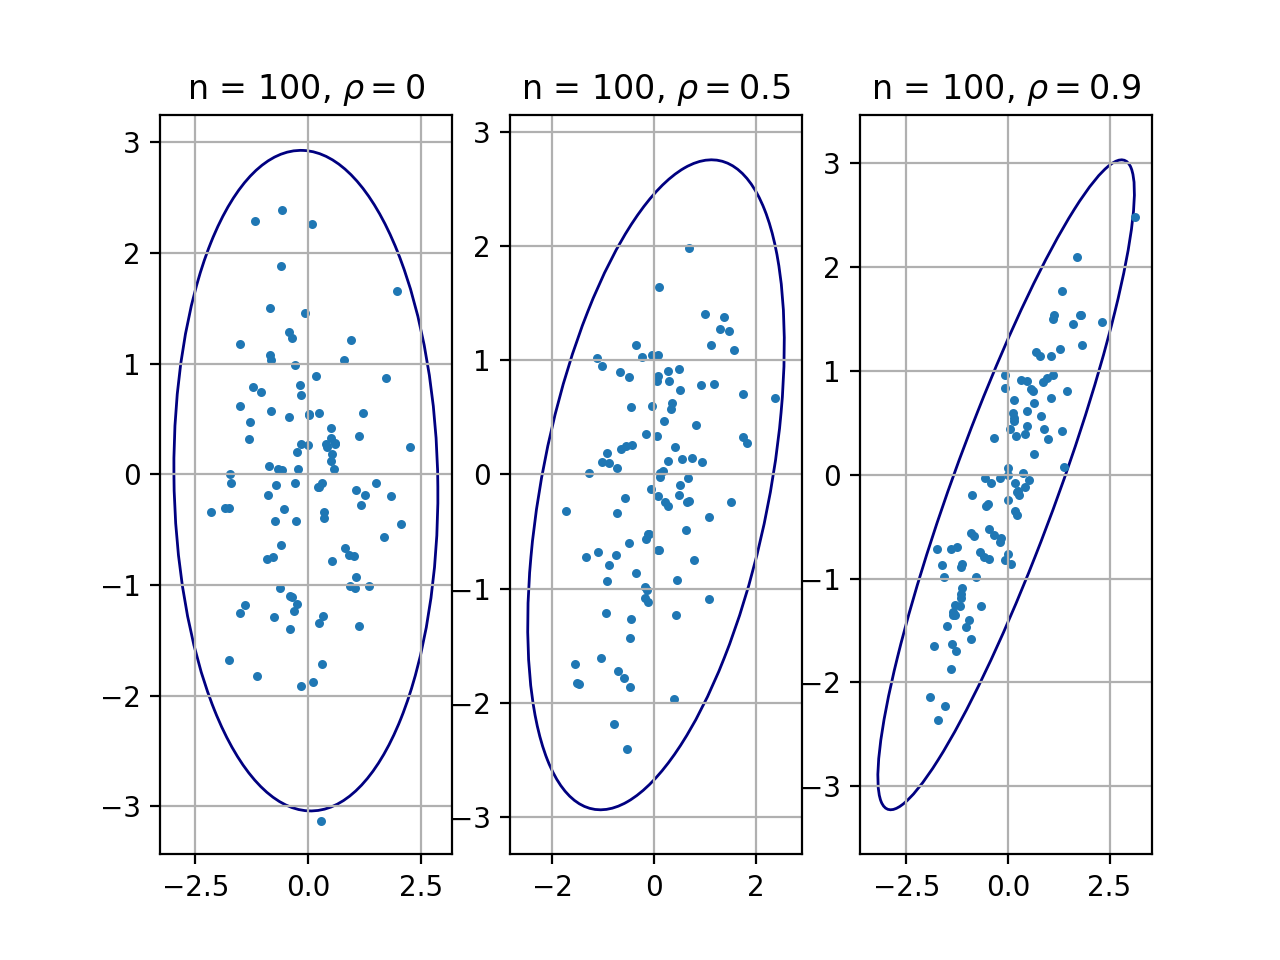
\includegraphics[width=1\linewidth]{task1\_data/100}}
	\caption{Двумерное нормальное распределение, $n$ = 100}
	\label{fig:n100}
\end{figure}
\begin{figure}[H]
	\center{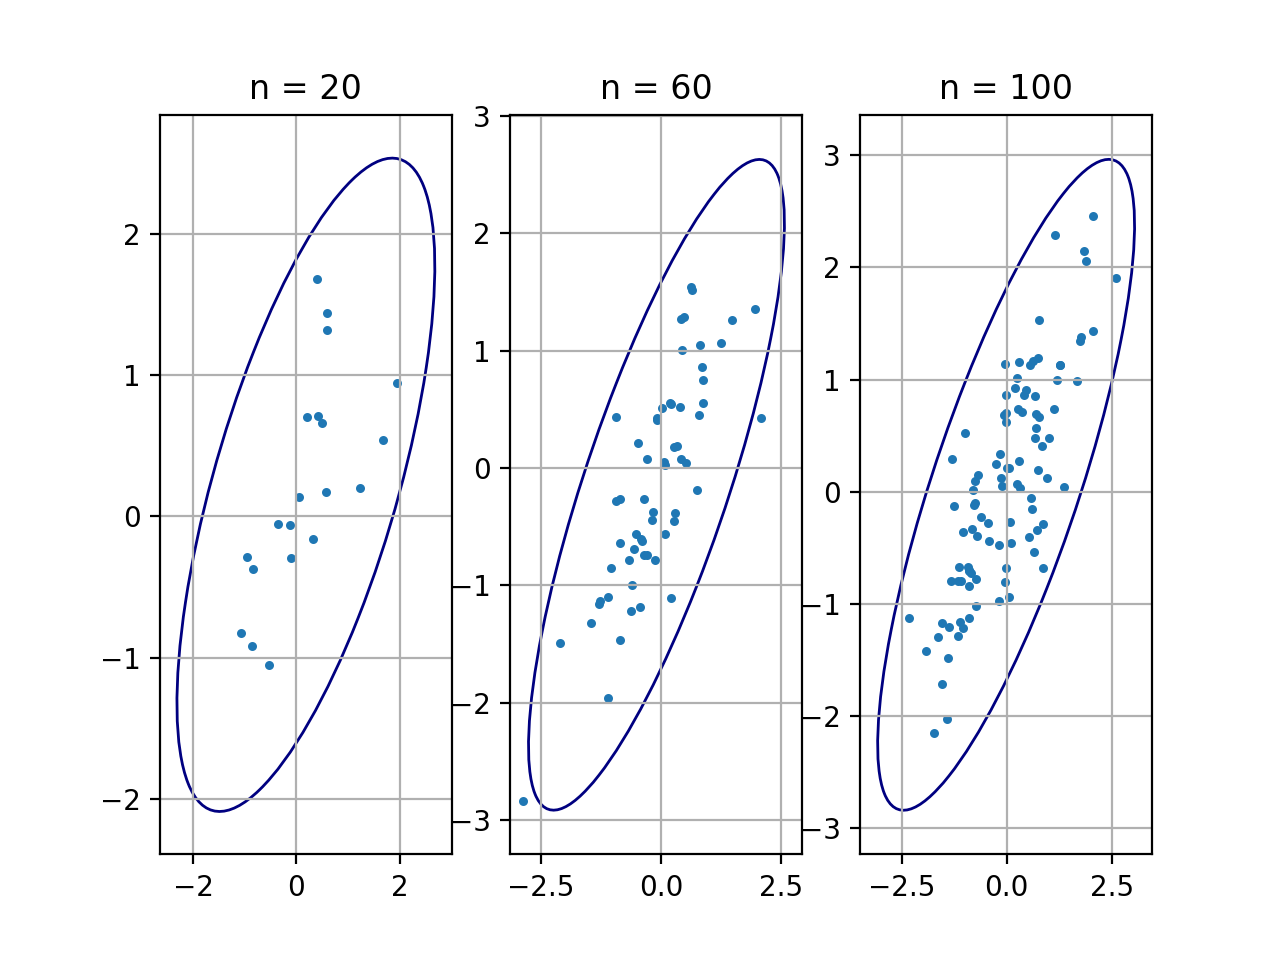
\includegraphics[width=1\linewidth]{task1\_data/mix}}
	\caption{Смесь нормальных распределений}
	\label{fig:mix}
\end{figure}

\subsection{Оценки коэффициентов линейной регрессии}
\subsubsection{Выборка без возмущений}
\begin{flushleft}
	\begin{enumerate}
\item Критерий наименьших квадратов:
$\hat{a}\approx 1.89$, $\hat{b}\approx 1.91$
\item Критерий наименьших модулей:
$\hat{a}\approx 2.00$, $\hat{b}\approx 1.70$
\end{enumerate}

\end{flushleft}
\begin{figure}[H]
	\center{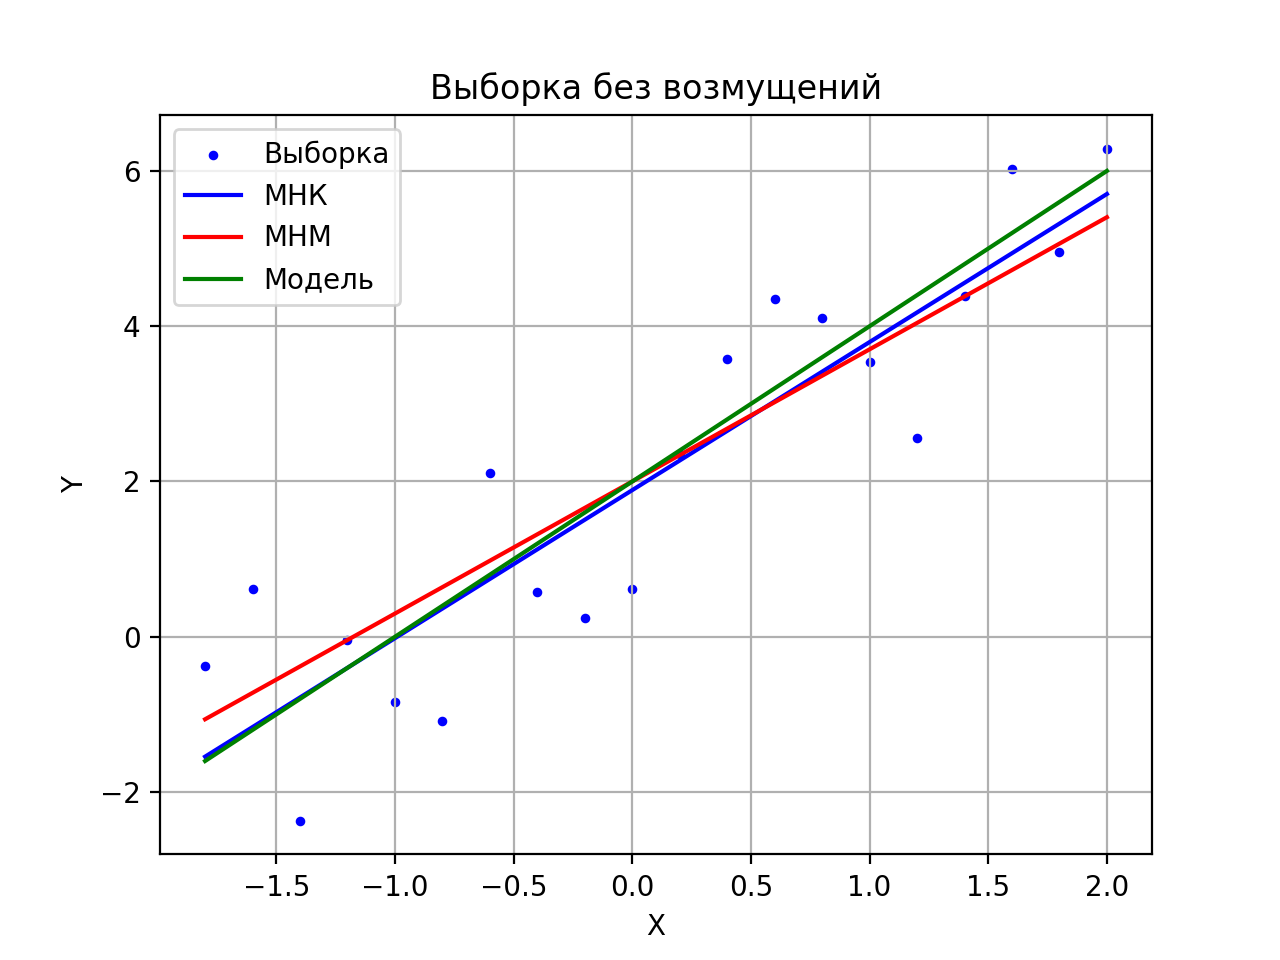
\includegraphics[width=1\linewidth]{task2\_data/no_noise}}
	\caption{Выборка без возмущений}
	\label{fig:no_noise}
\end{figure}
\subsubsection{Выборка с возмущениями}
\begin{flushleft}
	\begin{enumerate}
\item Критерий наименьших квадратов:
$\hat{a}\approx 2.03$, $\hat{b}\approx 0.48$
\item Критерий наименьших модулей:
$\hat{a}\approx 1.96$, $\hat{b}\approx 1.66$
\end{enumerate}

\end{flushleft}
\begin{figure}[H]
	\center{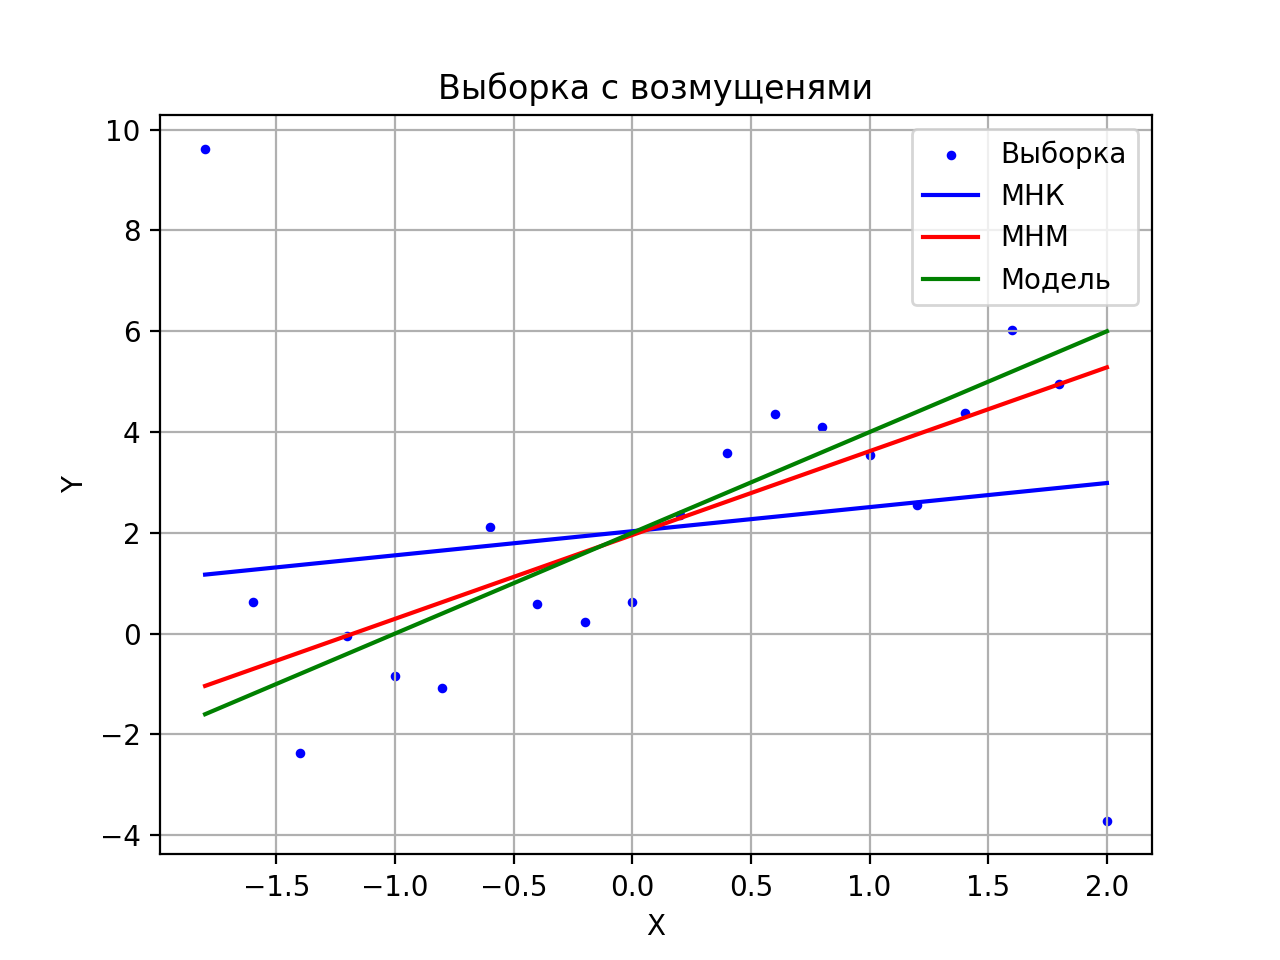
\includegraphics[width=1\linewidth]{task2\_data/noise}}
	\caption{Выборка с возмущениями}
	\label{fig:noise}
\end{figure}

\subsection{Проверка гипотезы о законе распределения генеральной совокупности. Метод хи-квадрат}
\begin{flushleft}
	Метод максимального правдоподобия: 
	$\hat{\mu} \approx -0.08, \hat{\sigma} \approx 0.96$\\
	\begin{table}[H]
		\centering
		\begin{tabular}{|c|c|c|c|c|c|c|}
\hline
\hline i & Границы $\Delta_i$ & $n_i$ & $p_i$ & $np_i$ & $n_i - np_i$ & $\frac{(n_i - np_i)^2}{np_i}$\\
\hline
1 & $-\infty$, -3.08 & 0.00 & 0.0009 & 0.09 & -0.09 & 0.09\\
\hline
2 & -3.08, -1.88 & 4.00 & 0.0291 & 2.91 & 1.09 & 0.41\\
\hline
3 & -1.88, -0.68 & 23.00 & 0.2353 & 23.53 & -0.53 & 0.01\\
\hline
4 & -0.68, 0.52 & 43.00 & 0.4695 & 46.95 & -3.95 & 0.33\\
\hline
5 & 0.52, 1.72 & 27.00 & 0.2353 & 23.53 & 3.47 & 0.51\\
\hline
6 & 1.72, 2.92 & 3.00 & 0.0291 & 2.91 & 0.09 & 0.00\\
\hline
7 & 2.92, $+\infty$ & 0.00 & 0.0009 & 0.09 & -0.09 & 0.09\\
\hline
$\sum$ & $-$ & 100.00 & 1.0000 & 100.00 & 0.00 & 1.44\\
\hline
\end{tabular}
		\caption{ Вычисление $\chi^{2}_{B}$ при проверке гипотезы $H_{0}$ о нормальном законе распределения $N(x,\hat{\mu}, \hat{\sigma})$}
		\label{tab:normal_chi_2}
	\end{table}
	Видим, что $\chi^{2}_{B} < \chi^{2}_{0.95} \approx 14.1$, следовательно, гипотезу полагаем верной.\\
	\begin{table}[H]
		\centering
		\begin{tabular}{|c|c|c|c|c|c|c|}
\hline
\hline i & Границы $\Delta_i$ & $n_i$ & $p_i$ & $np_i$ & $n_i - np_i$ & $\frac{(n_i - np_i)^2}{np_i}$\\
\hline
1 & $-\infty$, -3.16 & 0.00 & 0.0000 & 0.00 & -0.00 & 0.00\\
\hline
2 & -3.16, -1.96 & 0.00 & 0.0009 & 0.02 & -0.02 & 0.02\\
\hline
3 & -1.96, -0.76 & 5.00 & 0.1475 & 2.95 & 2.05 & 1.43\\
\hline
4 & -0.76, 0.44 & 13.00 & 0.7033 & 14.07 & -1.07 & 0.08\\
\hline
5 & 0.44, 1.64 & 2.00 & 0.1475 & 2.95 & -0.95 & 0.31\\
\hline
6 & 1.64, 2.84 & 0.00 & 0.0009 & 0.02 & -0.02 & 0.02\\
\hline
7 & 2.84, $+\infty$ & 0.00 & 0.0000 & 0.00 & -0.00 & 0.00\\
\hline
$\sum$ & $-$ & 20.00 & 1.0000 & 20.00 & 0.00 & 1.85\\
\hline
\end{tabular}
		\caption{Вычисление $\chi^{2}_{B}$ при проверке гипотезы $H_{0}$ о законе распределения $L(x,\hat{\mu}, \hat{\sigma})$, $n=20$}
		\label{tab:laplace_chi_2}
	\end{table}
	Видим, что $\chi^{2}_{B} < \chi^{2}_{0.95} \approx 14.1$, следовательно, гипотеза принимается и в этот раз.
\end{flushleft}

\subsection{Доверительные интервалы для параметров нормального распределения}
\begin{table}[H]
	\centering
	\begin{tabular}{| c | c | c |}
		\hline
		n = 20   &  $m$  & $\sigma$\\ \hline
		&  -0.38 < $m$ < 0.75 & 0.88 < $\sigma$ < 1.69 \\ \hline
		&   &   \\ \hline
		n = 100   &  $m$  & $\sigma$\\ \hline
		& -0.02 < $m$ < 0.40 & 0.95 < $\sigma$ < 1.25 \\
		\hline
	\end{tabular}
	\caption{Доверительные интервалы для параметров нормального распределения}
	\label{tab:interv_simple}
\end{table}

\subsection{Доверительные интервалы для параметров произвольного распределения. Асимптотический подход}
\begin{table}[H]
	\centering
	\begin{tabular}{| c | c | c |}
		\hline
		n = 20   &  $m$  & $\sigma$\\ \hline
		&  -0.29 < $m$ < 0.70 & 0.83 < $\sigma$ < 2.73 \\ \hline
		&   &   \\ \hline
		n = 100   &  $m$  & $\sigma$\\ \hline
		& -0.02 < $m$ < 0.40 & 0.90 < $\sigma$ < 1.42 \\
		\hline
	\end{tabular}
	\caption{Доверительные интервалы для параметров произвольного распределения. Асимптотический подход}
	\label{tab:interv_asimpt}
\end{table}

\subsection{Сравнение результатов 4.5 и 4.6. Графическое представление}
\begin{figure}[H]
	\center{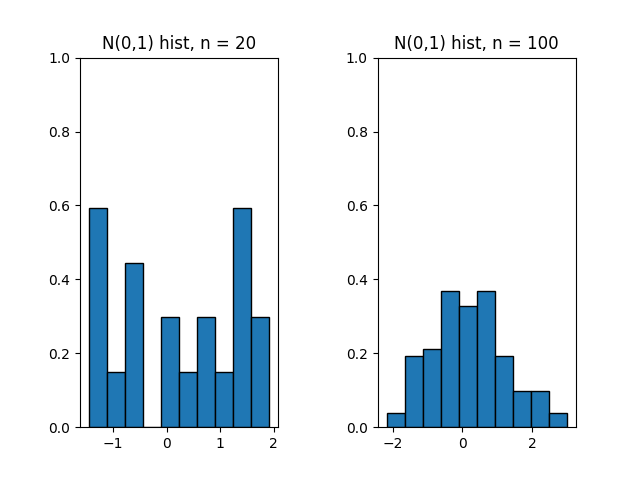
\includegraphics[width=1\linewidth]{task4\_data/hist}}
	\caption{Гистограмма распределения}
	\label{fig:hist}
\end{figure}
\begin{figure}[H]
	\center{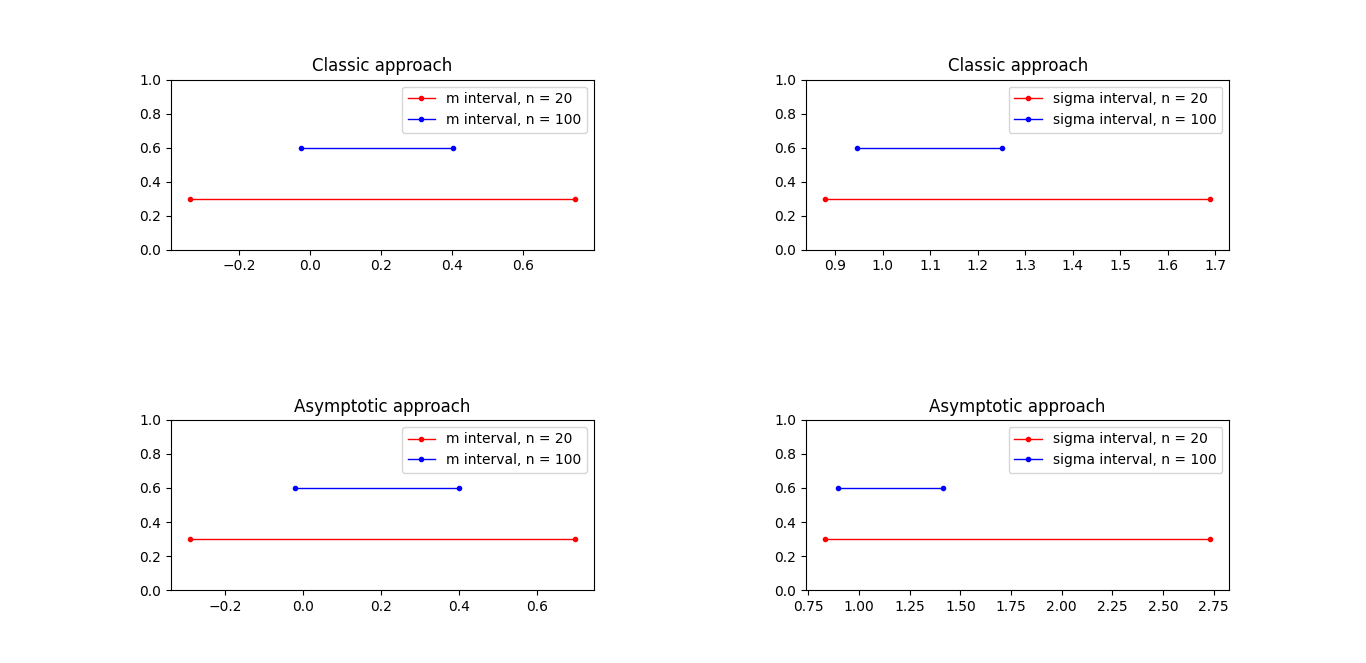
\includegraphics[width=1\linewidth]{task4\_data/intervals}}
	\caption{Полученные интервалы}
	\label{fig:intervals}
\end{figure}